%*************************************************************************************************************
%*************************************************************************************************************
%**************************Journal of Systems Science and Complexity (JSSC)***********************************
%*************************************************************************************************************
%*************************************************************************************************************
% This is the model of the standard format of articles published on Journal of Systems Science and Complexity.
% Please read through the whole guidance marked by "%" before you type according to the guidance.
% After "\end{document}", an article is attached just for an example and you can refer to it.
%*************************************************************************************************************

\documentclass{jssc}

%------------------------------------------------------------
\makeatletter
\def\@oddfoot{\hfill}
\newcount\shujiaocount
\def\setshujiao{%
  \shujiaocount=\count0
  \def\@oddfoot{%
      \ifodd\count0
         %\hfill\hbox to0pt{\hss\epsfig{figure=spr.eps,height=12pt}}
      \else
        %\epsfig{figure=spr.eps,height=12pt}
      \fi
  }%
}
%\catcode`@=\active
\makeatother

%************************************************************
%Beginning of the head of the tex file of JSSC. You can skip.
%************************************************************

%----------------------------------------------------------------------

\def\textsubscript#1%
{$_{\text{#1}}$}
\newcommand*\supercite[1]{\textsuperscript{\cite{#1}}}
%The definition of superscript about the cited references
\def\cdd{\mbox{\boldmath$\cdot$}~}
% name defs.tex
%\catcode`@=11
\def\vsp{\vspace{1mm}}
\def\no{\nonumber}
\def\q{\quad} \def\qq{\qquad}
\def\ee{{\rm e}}
\newcommand{\rulex}{\hfill\rule{1mm}{3mm}}
\def\ay{\arraycolsep=1.5pt}
\def\d{\displaystyle}
\def\dfrac{\displaystyle\frac}

%\input{amssym.def}
%\include{graphix}

%---------------------------------------------------------------------
%************************************************************
%End of the head of the tex file of JSSC.
%************************************************************


%%-------------------   Beginning of  Author's Definitions  -------------------%%
%%                     Note: You may add your own definitions here.

%************************************************************


%************************************************************
%Some user-defined commands, you can add more
%************************************************************
\usepackage{amsmath,amssymb}
\usepackage{pgf,tikz}
\usepackage{epstopdf}
\usetikzlibrary{shapes,arrows,automata}

\usepackage[noend,ruled]{algorithm2e}
\SetInd{2.7ex}{1.5ex}
\LinesNumbered
\SetKwBlock{Block}{begin}{end} \SetKwFor{While}{while}{do}{}
\SetKwFor{ForAll}{for all}{do}{} \SetKwFor{For}{for}{do}{}
\SetKwIF{If}{ElseIf}{Else}{if}{then}{else if}{else}{}
\newcommand{\KwAnd}{{\bf and}}
\newcommand{\Kwor}{{\bf or}}
\newcommand{\KwNot}{{\bf not}}
\SetAlgoSkip{medskip}

\newcommand{\rank}{{\rm rank}}
\newcommand{\while}{{\rm while}}
\newcommand{\oror}{{\rm or}}
\newcommand{\ifif}{{\rm if}}
\newcommand{\elif}{{\rm elseif}}
\newcommand{\then}{{\rm then}}
\newcommand{\els}{{\rm else}}
\newcommand{\head}{{\rm head}}
\newcommand{\tail}{{\rm tail}}
\newcommand{\A}{\mathcal{A}}
\newcommand{\I}{\mathcal{I}}
\newcommand{\J}{\mathcal{J}}
\newcommand{\V}{\mathcal{V}}
\newcommand{\define}{\hat{=}}
\newcommand{\xx}{\mathbf{x}}
\newcommand{\NTI}{{\bf NTI}}
\newcommand{\SNTI}{{\bf SNTI}}
\newcommand{\WNTI}{{\bf WNTI}}


%************************************************************

%%-------------------     the end of  Author's Definitions    -------------------%%


%*************************************************************************************************************
%*************************************************************************************************************
%*************************************************************************************************************
%***Beginning of the article! Please fill the content of your articles according to the guidance.
%*************************************************************************************************************
%*************************************************************************************************************
%*************************************************************************************************************
\setcounter{page}{1}
\input jsscN.tex
\begin{document}

%*************************************************************************************************************
% \biaoti{THE CAPITALIZED TITLE OF YOUR ARTICLE$^*$}{The list of authors' names with the LAST NAME capitalized
% and the authors' names should be separated by "\cdd"}{the first author's name \\ the first author's affiliation
% and Email address\\ the second author's name\\ the second author's affiliation. More can be listed like this.}
% {$^*$ The titles and numbers of the foundations that support this article.}
%*************************************************************************************************************
\biaoti{DISCOVERING NON-TERMINATING INPUTS FOR MULTI-PATH POLYNOMIAL PROGRAMS}%%%   Main Title of your paper  %%%
{LIU Jiang $\cdd$ XU Ming $\cdd$ ZHAN Naijun $\cdd$ ZHAO Hengjun}%%% The names of the authors  %%%
{LIU Jiang\\
{\it Chongqing Key Lab. of Automated Reasoning and Cognition, CIGIT, CAS, Chongqing, China}\\
E-mail\,$:$ liujiang@cigit.ac.cn\\
XU Ming\\
{\it Department of Computer Science and Technology, East China Normal University, Shanghai, China}\\
E-mail\,$:$ mxu@cs.ecnu.edu.cn\\
ZHAN Naijun\\
{\it State Key Lab. of Computer Science, Institute of Software, Chinese Academy of Sciences, Beijing, China}\\
E-mail\,$:$ znj@ios.ac.cn\\
ZHAO Hengjun (corresponding author)\\
{\it State Key Lab. of Computer Science, Institute of Software, Chinese Academy of Sciences, Beijing, China}\\
\& {\it University of Chinese Academy of Sciences}\\
E-mail\,$:$ zhaohj@ios.ac.cn}
%%% The address of the authors  %%%
{$^*$This research was supported by National Basic Research Program of China (No. 2014CB340700), National Science and Technology Major Project of China (No. 2012ZX01039-004), NSFC (Nos. 91118007, 11071273, 61202131), cstc2012ggB40004, SRFDP (No. 20130076120010), and the Open Project of Shanghai Key Lab. of Trustworthy Computing (No.~07dz22304201307).\\
{$^\diamond${\it This paper was recommended for publication by
Editor .... }}}

%*************************************************************************************************************
%The submission date of your article. For example: \drd{Received: June 8, 2006}
%*************************************************************************************************************
\drd{DOI: }{Received: x x 20xx}{ / Revised: x x 20xx}

%*************************************************************************************************************
% The page header of the article.
% \dshm{Year}{Volume}{The capitalized RUNNING HEAD of your article with less than 48 letters}{The capitalized
% AUTHORS list with $\cdot$ separating different names or one can type "The name of the first author et al."
% if there are more than 4 authors.}
%*************************************************************************************************************

\dshm{20XX}{XX}{DISCOVERING NON-TERMINATING INPUTS FOR MPPS}{LIU JIANG $\cdd$ XU MING $\cdd$ ZHAN NAIJUN $\cdd$ ZHAO HENGJUN}

%*************************************************************************************************************
% \dab{The abstract}{Keywords}
%*************************************************************************************************************
%-------------------------------------------------------------------------
\Abstract{We investigate the termination problems of multi-path polynomial programs (MPPs) with equational loop guards. To establish sufficient conditions for termination and nontermination simultaneously, we first propose the notion of strong/weak non-termination which under/over-approximates non-termination. Based on polynomial ideal theory, we show that the set of all strong non-terminating inputs (SNTI) and weak non-terminating inputs (WNTI) both correspond to the real varieties of certain polynomial ideals. Furthermore, we prove that the variety of SNTI is computable, and under some sufficient conditions the variety of WNTI is also computable. Then by checking the computed SNTI and WNTI varieties in parallel, termination properties of a considered MPP can be asserted. As a consequence, we establish a new framework for termination analysis of MPPs.}

\Keywords{termination analysis, polynomial programs, polynomial ideals.}        % the keywords

%\MRSubClass{68Q60, 68W30, 13F20}      % MR(2000) Subject Classification

%\baselineskip 15pt

\section{Introduction}
Termination analysis plays an important role in program verification and testing, and has attracted an increasing attention recently \cite{cook:termination,yang:advances}. However, the decision problem of program termination is equivalent to the famous halting problem \cite{turing:computable}, and hence is undecidable. Thus, a complete method for termination analysis for programs, even for the general linear or polynomial program, is impossible \cite{tiwari:terminate,bradley:polynomial,braverman:terminate}. To achieve positive results, a practical way analogous to \cite{Harris10} is to establish sufficient conditions for termination and nontermination simultaneously for a considered class of programs, and then check these conditions in parallel. We adopt this strategy of termination analysis in this work.

In this paper, we use multi-path polynomial programs (MPPs) as program models for termination analysis. The MPP model proposed in \cite{bradley:polynomial} is an expressive class of loops with multiple paths, polynomial loop guards and assignments, that enable practical code abstraction and analysis. It was proved in \cite{bradley:polynomial} that the termination problem of MPPs is generally undecidable. To get some computational results, we restrict to MPPs in the context whose loop guards are polynomial equations.

The semantics of an MPP with $\ell$ paths can be explained as follows. Given an input $\xx \in \mathbb{R}^n$, if at the first iteration $\xx$ satisfies the loop guard, then one of the multiple paths in the loop body will be nondeterministically selected and the corresponding assignment will be used to update the value of $\xx$, which results in $\ell$ possible values of $\xx$; at each following iteration, we repeat the same kind of loop guard test and nondeterministic assignment for each of the possible values of $\xx$ obtained so far. Thus the execution of an MPP on input $\xx \in \mathbb{R}^n$ produces a tree structure of execution paths, which is caused by the multi-paths in the considered program model.

An input $\xx$ is called a non-terminating input if the execution tree on $\xx$ has an infinite path. Given an MPP, we aim to compute an explicit representation for the set of all non-terminating inputs (NTI), or certain kinds of approximations of NTI. The theory of polynomial ideals serves as a critical tool for developing our approach.

The basic idea can be explained using a very simple example:
\[
\while \quad (G(x)=0) \quad \{x:=p(x);\} \enspace .
\]
The above MPP is composed of a single program variable $x$, the loop guard $G(x)=0$ and the polynomial assignments $p(x)$. If the MPP is non-terminating upon an input $x \in \mathbb{R}$, then $x,p(x),p(p(x)),\ldots$ must persistently satisfy $G(x)=0$, i.e. $G(x)=G(p(x))=G(p(p(x)))=\cdots=0$. Thus any non-terminating input is a common real root of the set of polynomials $\mathcal{G}\,\define\,\{G(x),G(p(x)),G(p(p(x))),\ldots\}$, or equivalently, an element in the real variety of the ideal $\I$ generated by $\mathcal{G}$. By a well-known result in polynomial ideal theory, $\I$ is generated by a finite number of elements in $\I$. If this finite set of generators of $\I$ can be computed, their common real roots comprise NTI.

For general MPPs with more than one paths, the NTI is not directly connected to the real variety of a polynomial ideal. Instead, we propose the notions of strong and weak non-termination, such that the set of all strong non-terminating inputs (SNTI) is a \emph{subset} of NTI, and the set of all weak non-terminating inputs (WNTI) is a \emph{superset} of NTI. Therefore the non-emptiness of SNTI is a sufficient condition for non-termination, and the emptiness of WNTI is a sufficient condition for termination. Furthermore, both SNTI and WNTI are shown to be real varieties of certain polynomial ideals, of which a finite set of generators can be computed (at least under some sufficient conditions). Thus for any MPP, its SNTI and WNTI can be investigated simultaneously for a better result of termination analysis. The proposed approach will be illustrated by some examples.

\subsection{Related work}
In the past, most well-established work on termination analysis can only be applied to linear programs, whose guards and assignments are linear. A classical method for establishing termination of a program, either linear or polynomial, makes use of a well-founded domain together with the so-called \emph{ranking function} that maps the state space of the program to the domain. For single-path linear programs, Col\'{o}n and Sipma utilized polyhedral cones to synthesize linear ranking functions \cite{colon:synthesis}. Podelski and Rybalchenko, based on Farkas' lemma, presented a complete method to find linear ranking functions if they exist \cite{podelski:ranking}. These methods pay more attention to the search for ranking functions than to the inherent structure of loops, while Tiwari first noticed that the termination of a class of simple linear loops is closely related to the eigenvalues of assignment matrix, and proved that the termination problem of linear programs is decidable over $\mathbb{R}$ \cite{tiwari:terminate}. This theory was further developed by Braverman \cite{braverman:terminate} and Xia et al \cite{XZ2010,XYZZ2011}. Xu et~al also developed Tiwari's work by constructing non-terminating witnesses \cite{xu:terminate,XuL13}.

It was shown in \cite{bradley:polynomial} that the termination of MPPs is undecidable by reduction from Diophantine equations. However, effective methods that are incomplete or relatively complete for analyzing termination still exist. Bradley et~al. proposed an approach to proving termination over $\mathbb{R}$ through finite difference trees \cite{bradley:polynomial}. Cook et~al. \cite{cook:conditional} devised an algorithm to under-approximate the \emph{weakest preconditions} for termination using decidable theories. Typically, with the development of computer algebra, more and more techniques from symbolic computation, for instance, Gr\"{o}bner basis \cite{sank:GB,muller:invariants}, quantifier elimination \cite{kapur:QE} and recurrence relation \cite{rodriguez:simple,kovacs:psolvable}, are borrowed and successfully applied to the verification of  programs. Certainly, these techniques can also be applied to polynomial programs to discover termination or non-termination proofs. Chen et~al. proposed a relatively complete (w.r.t. a given template) method for generating polynomial ranking functions over $\mathbb{R}$ by reduction to semi-algebraic system solving \cite{chen:ranking}. On the other hand, Gupta et~al. proposed a practical method to search for counter-examples of termination \cite{gupta:NT}, by first generating lasso-shaped \cite{cook:code} candidate paths and then checking the feasibility of the ``lassoes" using constraint solving. Velroyen and R\"{u}mmer applied invariants to show that terminating states of a program are unreachable from certain initial states, and then identified these ``bad'' initial states by constraint-solving techniques \cite{Velroyen08}. Brockschmidt et~al. detected non-termination and Null Pointer Exceptions for \textsf{Java Bytecode} by constructing and analyzing termination graphs, and implemented a termination prover \textsf{AProVE} \cite{Brockschmidt11}.

For more general programs, many other techniques, like predicate abstraction, parametric abstraction, fair assumption, Lagrangian relaxation, semidefinite programming, sum of squares and curve fitting \cite{cousot:lagrangian,shen:curve}, and so on, have been successfully applied.

\paragraph{Organization}
The remainder of this paper is organized as follows. In Section~\ref{sec:prel}, some concepts and results on polynomial ideals are reviewed. In Section~\ref{sec:MPP}, we first introduce MPPs and then define the notions of non-termination, strong/weak non-termination. In Sections~\ref{sec:snt} and \ref{sec:wnt} we show how to compute the set of all strong and weak non-terminating inputs of MPPs respectively. Finally we draw a conclusion in Section~\ref{sec:conc}.

\section{Preliminaries}\label{sec:prel}
In this section, we briefly recall some basic concepts and results on computational algebraic geometry, which serve as the theoretical tool for dealing with non-terminating inputs. For a detailed exposition to this subject, please refer to \cite{cox:ideal}. Throughout this paper, we use $\mathbb{N}, \mathbb{Q}, \mathbb{R}$ to denote the set of natural, rational, and real numbers, respectively.

\begin{definition}[Ideal]
Let $\xx=(x_1,x_2,\ldots,x_n)$ be a vector of variables. A subset $\I$ of the polynomial ring $\mathbb{Q}[\xx]$ is an \emph{ideal} if it satisfies:
\begin{itemize}
\item[(i)] $0 \in \I$;
\item[(ii)] if $p,q \in \I$, then $p+q \in \I$;
\item[(iii)] if $p \in \I$ and $r \in \mathbb{Q}[\xx]$, then $rp \in \I$.
\end{itemize}
\end{definition}

\begin{definition}[Variety]
Given a field $\mathbb{K}$ extending $\mathbb{Q}$, the \emph{variety} defined by $P \subseteq \mathbb{Q}[\xx]$ is $\V(P)=\{\xx \in \mathbb{K}^n \ | \ \forall \ p \in P \ : \ p(\xx)=0 \}$. The \emph{real variety} of $P$ is the intersection of $\V(P)$ and $\mathbb{R}^n$, i.e., $\V(P) \cap \mathbb{R}^n$.
\end{definition}

Let $P$ be a nonempty subset of $\mathbb{Q}[\xx]$. It is easy to verify that
\[
\left\{\sum_{i=1}^k r_i p_i \ | \ k \in \mathbb{N}, \ r_i \in \mathbb{Q}[\xx],\ p_i \in P \right\}
\]
is an ideal, denoted by $\langle P\rangle$, and $P$ is called a set of \emph{generators}, or a \emph{basis} of $\langle P \rangle$. In particular, if $P$ is a finite set $\{p_1,p_2,\ldots,p_k\}$, then $\langle P \rangle$ is written as $\langle p_1,p_2,\ldots,p_k \rangle$. An ideal $\I$ is called \emph{principal} if it can be generated by a single element, i.e., $\I=\langle p \rangle$ for some $p\in \mathbb{Q}[\xx]$. It is easy to verify that $\V(P)=\V(\langle P \rangle)$ for any $P \subseteq \mathbb{Q}[\xx]$.

\begin{theorem}[Hilbert's Basis Theorem]\label{basis}
Every ideal $\I \subseteq \mathbb{Q}[\xx]$ has a finite number of generators, i.e., $\I=\langle p_1,p_2,\ldots,p_k \rangle$ for some $p_1,p_2,\ldots,p_k \in \I$.
\end{theorem}

In particular, for any $\I=\langle p_1,p_2,\ldots,p_k \rangle$, a unique \emph{(reduced) Gr\"{o}bner basis} of $\I$ can be computed using Buchberger's algorithm, under a fixed \emph{monomial ordering}. Using Gr\"{o}bner basis, the problems of deciding membership of an element in an ideal, testing equality or inclusion of ideals, and so on, can be effectively solved; a Gr\"obner basis is also helpful in checking whether a given ideal is principal.

Given an ideal $\I=\langle p_1,p_2,\ldots,p_k \rangle$, by applying so-called real-solution-isolation algorithms \cite{xia:SAS,xia:DISCOVERER} to the system of polynomial equations $p_i(\xx)=0$ for $1 \leq i \leq k$, the emptiness of the real variety $\V(\I) \cap \mathbb{R}^n$ can be checked; and if it is nonempty and is zero-dimensional, the finite set of points in $\V(\I) \cap \mathbb{R}^n$ can be isolated using arbitrarily small cubes (with rational endpoints).

All the above mentioned algorithms have been well-implemented in the computer algebra system {\sc Maple}.

The following result can be derived from Hilbert's Basis Theorem.

\begin{theorem}[The Ascending Chain Condition]\label{ascending}
Let $\I_1 \subseteq \I_2 \subseteq \I_3 \subseteq \cdots$ be an ascending chain of ideals in $\mathbb{Q}[\xx]$. Then there exists an integer $N$ such that $\I_N=\I_{N+1}=\I_{N+2}=\cdots$.\footnotemark \footnotetext{Here $\I_N$ is called the \emph{fixed point} of this chain.}
\end{theorem}


\section{Multi-path Polynomial Programs and Non-termination}\label{sec:MPP}
\subsection{Multi-path Polynomial Programs}
\begin{definition}[MPP with Equational Loop Guard]
A \emph{multi-path polynomial program} with \emph{equational} loop guard and $\ell$ paths is of the form
\begin{equation}\label{eqn:MPP}
\while \quad (G(\xx)=0) \quad \left\{
\begin{array}{ll}
   & \quad \xx:= {\bf A}_1(\xx); \\
|| & \quad \xx:= {\bf A}_2(\xx); \\
   & \quad \vdots \\
|| & \quad \xx:= {\bf A}_{\ell-1}(\xx); \\
|| & \quad \xx:= {\bf A}_{\ell}(\xx); \\
\end{array}
\right\} \enspace ,
\end{equation}
where
\begin{itemize}
\item $\xx \in \mathbb{R}^n$ denotes a vector of program variables;
\item $G(\xx) \in \mathbb{Q}[\xx]$ is a polynomial and $G(\xx)=0$ is the equational loop guard;
\item ``$||$'' interprets an {\it exclusive choice} of the $\ell$ paths;
\item ${\bf A}_i \in \mathbb{Q}^n[\xx]$ for $1 \leq i \leq \ell$ corresponding to each path is a vector of polynomials describing \emph{simultaneous} assignments for all program variables.
\end{itemize}

\end{definition}
Note that
\begin{enumerate}
\item[1)] MPP~(\ref{eqn:MPP}) allows arbitrary Boolean combinations of polynomial equations of the form $\bigvee_{i=1}^M \bigwedge_{j=1}^{N_i} G_{ij}(\xx)=0$ as loop guard, and assuming $G(\xx)=0$ would not lose any generality, since
    \begin{equation}\label{eqn:guard}
    \left[ \bigvee_{i=1}^M \bigwedge_{j=1}^{N_i} G_{ij}(\xx) = 0 \right]  \Longleftrightarrow \left[ \prod_{i=1}^M \sum_{j=1}^{N_i} [G_{ij}(\xx)]^2 = 0 \right] \enspace .
    \end{equation}
\item[2)] Initial conditions on $\xx$ are not specified, since we are aiming to compute the set of all non-terminating inputs (as real varieties) for a given MPP; nevertheless, equational initial conditions on $\xx$ can be easily taken into account by manipulation of corresponding ideals.
\end{enumerate}

\begin{example}
Consider the following MPP
\[
\begin{array}{l}
\while \quad (x-z^3=0 \vee y-z^2=0) \\
\qquad \left\{
\begin{array}{ll}
 & \quad (x,y,z) := (x,y+2z+1,z+1); \\
|| & \quad (x,y,z) := (x-3y+3z-1,y+2z-1,z-1); \\
\end{array}
\right\} \enspace  .\\
\end{array}
\]
According to (\ref{eqn:guard}), the loop guard $y-z^2=0 \vee x-z^3=0$ can be transformed to $(x-z^3)^2 \times (y-z^2)^2=0$, or equivalently $(x-z^3) \times (y-z^2)=0$. There are two exclusive simultaneous assignments, i.e., $(x,y,z):=(x,y+2z+1,z+1)$ and $(x,y,z):=(x-3y+3z-1,y+2z-1,z-1)$, which can be named by ${\bf A}_1$ and ${\bf A}_2$ in the manner of MPP~(\ref{eqn:MPP}). \rulex
\end{example}

\subsection{The Execution of MPPs}
We associate with each ${\bf A}_i$ in MPP~(\ref{eqn:MPP}) a different symbol $a_i$ indexed by $i$ for $1 \leq i \leq \ell$. Then the execution of MPP~(\ref{eqn:MPP}) on input $\xx \in \mathbb{R}^n$ can be graphically represented as a \emph{labeled execution tree} illustrated by Figure~\ref{fig:exe-tree}. The nodes in the execution tree are elements in $\mathbb{R}^n$. A directed edge labeled by $a_i$ stands for the execution of assignment ${\bf A}_i$, and points to the updated value given by the execution of ${\bf A}_i$. Formally,
\begin{definition}[Execution Tree]
The \emph{execution tree} is defined inductively as:
\begin{itemize}
\item the \emph{root} is $\xx$;
\item for any node $\xx'$ in the tree, it is a \emph{leaf node} if $G(\xx') \neq 0$; otherwise $\xx'$ has $\ell$ \emph{children} ${\bf A}_1(\xx'), {\bf A}_2(\xx'), \ldots, {\bf A}_{\ell}(\xx')$, and there is a \emph{directed edge} connecting $\xx'$ and ${\bf A}_i(\xx')$, labeled by $a_i$, for any $1 \leq i \leq \ell$.
\end{itemize}
\end{definition}

\begin{figure}
\begin{minipage}[t]{0.5\linewidth}
\centering
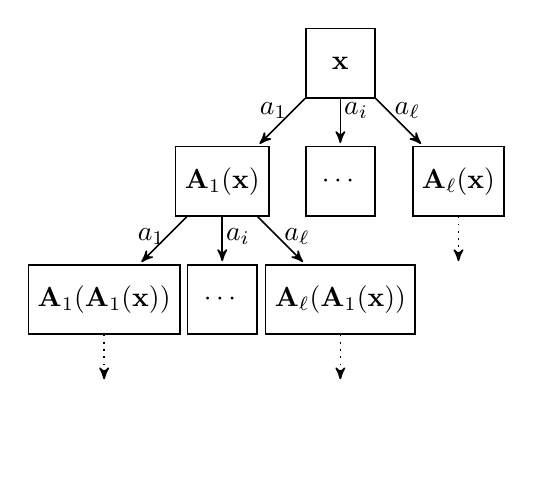
\begin{tikzpicture}[->,>=stealth',shorten >=1pt,auto,node distance=1.5cm,semithick]
\node[state,rectangle](q1){$\xx$};
\node[state,rectangle](q3)[below of=q1]{$\cdots$};
\node[state,rectangle](q2)[left of=q3]{${\bf A}_1(\xx)$};
\node[state,rectangle](q4)[right of=q3]{${\bf A}_{\ell}(\xx)$};
\node[state,rectangle](q6)[below of=q2]{$\cdots$};
\node[state,rectangle](q5)[left of=q6]{${\bf A}_1({\bf A}_1(\xx))$};
\node[state,rectangle](q7)[right of=q6]{${\bf A}_{\ell}({\bf A}_1(\xx))$};

\node[state,rectangle,white](q8)[below of=q4]{};
\node[state,rectangle,white](q9)[below of=q5]{};
\node[state,rectangle,white](q10)[below of=q7]{};

\draw[->](q1)edge[swap](q2); \draw[->](q1)edge[swap](q3);
\draw[->](q1)edge[swap](q4); \draw[->](q2)edge[swap](q5);
\draw[->](q2)edge[swap](q6); \draw[->](q2)edge[swap](q7);
\draw[->](q4)edge[swap,dotted](q8);
\draw[->](q5)edge[swap,dotted](q9);
\draw[->](q7)edge[swap,dotted](q10);

\node at (-.85,-.6) {$a_1$};
\node at (.2,-.6) {$a_i$};
\node at (.85,-.6) {$a_{\ell}$};
\node at (-2.4,-2.2) {$a_1$};
\node at (-1.3,-2.2) {$a_i$};
\node at (-.55,-2.2) {$a_{\ell}$};

\end{tikzpicture}
\caption{\small The labeled execution tree of MPP~(\ref{eqn:MPP}) on input $\xx$}\label{fig:exe-tree}
\end{minipage}
\hspace{.5cm}
\begin{minipage}[t]{0.45\linewidth}
\centering
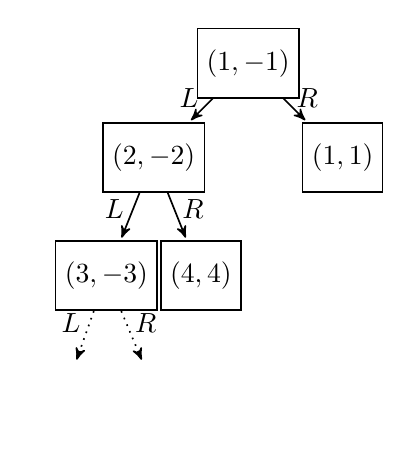
\begin{tikzpicture}[->,>=stealth',shorten >=1pt,auto,node distance=1.2cm,semithick]
\node[state,rectangle](q1){$(1,-1)$};
\node[state,rectangle,white](q3)[below of=q1]{};
\node[state,rectangle](q2)[left of=q3]{$(2,-2)$};
\node[state,rectangle](q4)[right of=q3]{$(1,1)$};

\node[state,rectangle](q6) at (-.6,-2.7) {$(4,4)$};
\node[state,rectangle](q5)[left of=q6]{$(3,-3)$};

\node[state,rectangle,white](q9) at (-2.35,-4.25) {$0$};
\node[state,rectangle,white](q10)[right of=q9]{$2$};

\draw[->](q1)edge[swap](q2);
\draw[->](q1)edge[swap](q4);
\draw[->](q2)edge[swap](q5);
\draw[->](q2)edge[swap](q6);

\draw[->](q5)edge[swap,dotted](q9);
\draw[->](q5)edge[swap,dotted](q10);

\node at (-.75,-.45) {$L$};
\node at (.75,-.45) {$R$};
\node at (-1.7,-1.85) {$L$};
\node at (-0.7,-1.85) {$R$};
\node at (-2.25,-3.3) {$L$};
\node at (-1.3,-3.3) {$R$};
\end{tikzpicture}

\caption{\small The execution tree of MPP~(\ref{eqn:eg-exe-path}) on input $(1,-1)$}\label{fig:exe-path}
\end{minipage}
\end{figure}

To characterize the set of paths in Figure~\ref{fig:exe-tree} starting from root $\xx$, we introduce below some conventional notions on \emph{alphabet} and \emph{strings} for self-containedness.

Let $\Sigma$ be a finite set of symbols, called an \emph{alphabet}. A finite or infinite \emph{string} over $\Sigma$ can be denoted respectively by $\tau=a_1a_2 \cdots a_s$ or $\tau=a_1a_2 \cdots a_s a_{s+1} \cdots$, where $a_i \in \Sigma$ for $i=1,2,\ldots$. A string without any symbol is called the \emph{empty string}, denoted by $\epsilon$. We identify strings with one symbol as the symbol itself. By convention, the set of all finite (including $\epsilon$) and infinite strings are denoted by $\Sigma^*$ and $\Sigma^{\omega}$, respectively.
Let $|\tau|$ denote the length of a string $\tau$. Thus $|\epsilon|=0$, $|\tau|=s$ if $\tau=a_1 a_2 \cdots a_s$, and $|\tau|=\infty$ if $\tau \in \Sigma^{\omega}$. Given $\tau \in \Sigma^* \cup \Sigma^{\omega}$, if there exist $\tau_1 \in \Sigma^*$ and $\tau_2 \in \Sigma^* \cup \Sigma^{\omega}$ such that $\tau = \tau_1 \cdot \tau_2$, where $\cdot$ is the \emph{concatenation} operator on strings, then $\tau_1$ is called a \emph{prefix} of $\tau$; if in addition $|\tau_1|=1$, then $\tau_1$ and $\tau_2$ are called the \emph{head} and \emph{tail} of $\tau$, denoted by $\head(\tau)$ and $\tail(\tau)$ respectively. The set of all prefixes of $\tau$ is denoted by ${\bf Pre}(\tau)$; if $\tau' \in {\bf Pre} (\tau)$ and $\tau' \neq \tau$, then $\tau'$ is called a \emph{proper} prefix of $\tau$.

Let $\Sigma$ be the alphabet consists of all the labels in Figure~\ref{fig:exe-tree}, i.e., $\Sigma=\{a_1,a_2,\ldots,a_{\ell}\}$. Then for any path in Figure~\ref{fig:exe-tree} from root $\xx$ to some node $\xx'$, the labels of the edges along this path generate a finite string $\tau$ over $\Sigma$; furthermore, $\xx'$ results from $\xx$ by the iterated application of the assignments corresponding to the symbols appearing in $\tau$.

Actually, if we define an induced function $\A_{\tau}: \mathbb{R}^n \rightarrow \mathbb{R}^n$ for any $\tau\in \Sigma^*$ as:
\begin{itemize}
\item $\A_{\epsilon}={\bf id}$, i.e., the identity mapping;
\item $\A_{a_i}={\bf A}_i$ for any $a_i\in \Sigma$, where ${\bf A}_i$ is the $i$-th assignment in MPP~(\ref{eqn:MPP});
\item $\A_{\tau} = \A_{\tail(\tau)} \circ \A_{\head(\tau)}$ for $\tau$ with $|\tau|\geq 2$, where $\circ$ denotes the \emph{composition} of functions, i.e., $(f \circ g)(\xx)=f(g(\xx))$ for $f,g: \mathbb{R}^n \rightarrow \mathbb{R}^n$,
\end{itemize}
then the set of paths starting from root $\xx$ of the labeled tree in Figure~\ref{fig:exe-tree} can be represented by a set of strings over $\Sigma$, using the following definition.

\begin{definition}[Execution Path]\label{dfn:exe-path}
Let $\Sigma$ be what specified above for MPP~(\ref{eqn:MPP}). Then $\tau \in \Sigma^* \cup \Sigma^{\omega}$ is an \emph{execution path} of MPP~(\ref{eqn:MPP}) on input $\xx \in \mathbb{R}^n$ if
\begin{itemize}
\item $\tau=\epsilon$; or
\item $G(\A_{\tau'}(\xx))=0$ for all $\tau' \in {\bf Pre}(\tau), \tau' \neq \tau$ (i.e., $\tau'$ is a proper prefix of $\tau$).
\end{itemize}
\end{definition}

We denote the set of all execution paths of MPP~(\ref{eqn:MPP}) on input $\xx$ by ${\bf Path}(\xx)$. Then there is a one-to-one correspondence between ${\bf Path}(\xx)$ and the set of paths from root $\xx$ in Figure~\ref{fig:exe-tree}: for any execution path $\tau=a_1a_2 \cdots a_s \cdots$ (finite or infinite), there is a path in Figure~\ref{fig:exe-tree} from $\xx$ to a node $\A_{\tau}(\xx)$,  labeled by the symbols $a_1,a_2,\ldots,a_s,\ldots$; conversely, for any path from $\xx$ to some node $\xx'$ in Figure~\ref{fig:exe-tree}, the juxtaposition of the labels along this path gives an execution path in ${\bf Path}(\xx)$.

\begin{example}\label{eg:exe-path}
Consider the following MPP
\begin{equation}\label{eqn:eg-exe-path}
\while \quad (x+y=0) \quad \left\{
\begin{array}{ll}
& \quad (x,y) := (x+1, y-1); \\
\,|| & \quad (x,y) := (x^2, y^2); \\
\end{array}
\right\}
\enspace .
\end{equation}
If we associate symbols $L,R$ with the first and second assignments of MPP~(\ref{eqn:eg-exe-path}) respectively, it is easy to verify that on input $(1,-1)$, MPP~(\ref{eqn:eg-exe-path}) has an infinite execution path $LLL \cdots$ and finite execution paths $R,LR,LLR$ and so on (see Figure~\ref{fig:exe-path}). \rulex
\end{example}

\subsection{Non-termination Definitions}
\begin{definition}[Non-termination]\label{def:Termin}
An input $\xx \in \mathbb{R}^n$ of MPP~(\ref{eqn:MPP}) is a {\em non-terminating input} if the MPP has an infinite execution path on $\xx$, i.e., ${\bf Path}(\xx) \cap \Sigma^{\omega} \neq \emptyset$; otherwise $\xx$ is a \emph{terminating input}.
\end{definition}

\begin{example}\label{eg:nt}
Consider MPP~(\ref{eqn:eg-exe-path}). By Example~\ref{eg:exe-path}, MPP~(\ref{eqn:eg-exe-path}) has an infinite execution path $LLL \cdots$ on $(1,-1)$. So $(1,-1)$ is a non-terminating input of MPP~(\ref{eqn:eg-exe-path}). \rulex
\end{example}

The set of all non-terminating inputs of MPP~(\ref{eqn:MPP}) is denoted by $\NTI$. Termination analysis of MPPs concerns such problems as
\begin{enumerate}
\item[1)] whether a given MPP terminates on all inputs $\xx$; or alternatively,
\item[2)] detection of non-terminating inputs for a given MPP.
\end{enumerate}
It was proved in \cite{bradley:polynomial} that for general MPPs with inequality-typed loop guards, the problem of deciding whether $\NTI$ is an empty set is undecidable. To get some computational results for termination analysis of MPP~(\ref{eqn:MPP}), we propose the following two notions for under/over-approximating non-terminating input set.

\begin{definition}[Strong Non-termination]\label{def:SNT}
An input $\xx \in \mathbb{R}^n$ of MPP~(\ref{eqn:MPP}) is a \emph{strong} non-terminating input if the MPP has all the infinite strings as its execution paths, i.e., $\Sigma^{\omega} \subseteq {\bf Path}(\xx)$.
\end{definition}

Intuitively, on a strong nonterminating input, the loop guard of MPP~(\ref{eqn:MPP}) is persistently satisfied no matter how many iterations have been executed, or which assignment is selected at each iteration.

\begin{example}\label{eg:snt}
Consider the following MPP
\begin{equation}\label{eqn:eg-snt}
\while \quad (x^2+1-y=0) \quad \left\{
\begin{array}{ll}
& \quad (x,y) := (x,x^2y); \\
\,|| & \quad (x,y) := (-x,y); \\
\end{array}
\,\right\} \enspace .
\end{equation}
We associate symbols $L,R$ with the two assignments in MPP~(\ref{eqn:eg-snt}) respectively. Figure~\ref{fig:eg-snt} illustrates the execution tree of MPP~(\ref{eqn:eg-snt}) on input $(1,2)$. Note that both $(1,2)$ and $(-1,2)$ satisfy the loop guard. So it can be shown that $(1,2)$ is a strong non-terminating input of MPP~(\ref{eqn:eg-snt}). \rulex
\end{example}

\begin{definition}[Weak Non-termination]\label{def:WNT}
An input $\xx \in \mathbb{R}^n$ of MPP~(\ref{eqn:MPP}) is a \emph{weak} non-terminating input if for any $k \in \mathbb{N}$, there exists $\tau_k \in\Sigma^*$ such that
\begin{equation}\label{eqn:wnt}
|\tau_k|=k \,\mbox{ and }\, G(\A_{\tau_k}(\xx))=0 \enspace.
\end{equation}
\end{definition}

Intuitively, on a weak nonterminating input $\xx$, we can find $\tau_k$ of any length $k \in \mathbb{N}$, such that when applying the induced function $\A_{\tau_k}$ to $\xx$, the loop guard will be satisfied. However, as the set of such $\tau_k$ is not \emph{prefix-closed}, according to Definition~\ref{dfn:exe-path}, $\tau_k$ is not necessarily an execution path for any $k$. Therefore we call such $\tau_k$ \emph{pseudo execution paths} of MPP~(\ref{eqn:MPP}).

\begin{figure}
\begin{minipage}[t]{0.45\linewidth}
\centering
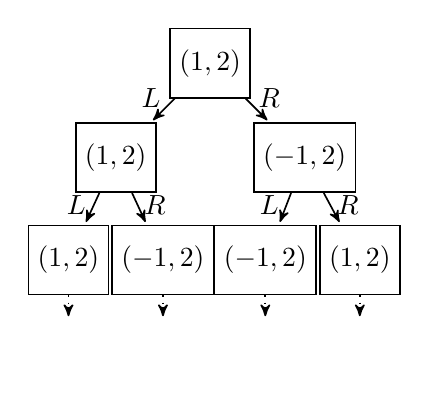
\begin{tikzpicture}[->,>=stealth',shorten >=1pt,auto,node distance=1.2cm,semithick]
\node[state,rectangle](q1){$(1,2)$};
\node[state,rectangle,white](q3)[below of=q1]{};
\node[state,rectangle](q2)[left of=q3]{$(1,2)$};
\node[state,rectangle](q4)[right of=q3]{$(-1,2)$};

\node[state,rectangle](q6) at (-.6,-2.5) {$(-1,2)$};
\node[state,rectangle](q5)[left of=q6]{$(1,2)$};
\node[state,rectangle](q7) at (0.7,-2.5) {$(-1,2)$};
\node[state,rectangle](q8)[right of=q7]{$(1,2)$};

\node[state,rectangle,white](q9)[below of=q5]{$(1,2)$};
\node[state,rectangle,white](q10)[below of=q6]{$(-1,2)$};
\node[state,rectangle,white](q11)[below of=q7]{$(-1,2)$};
\node[state,rectangle,white](q12)[below of=q8]{$(1,2)$};

\draw[->](q1)edge[swap](q2);
\draw[->](q1)edge[swap](q4);
\draw[->](q2)edge[swap](q5);
\draw[->](q2)edge[swap](q6);
\draw[->](q4)edge[swap](q7);
\draw[->](q4)edge[swap](q8);

\draw[->](q5)edge[swap,dotted](q9);
\draw[->](q6)edge[swap,dotted](q10);
\draw[->](q7)edge[swap,dotted](q11);
\draw[->](q8)edge[swap,dotted](q12);

\node at (-.75,-.45) {$L$};
\node at (.75,-.45) {$R$};
\node at (-1.7,-1.8) {$L$};
\node at (-0.7,-1.8) {$R$};
\node at (1.75,-1.8) {$R$};
\node at (0.75,-1.8) {$L$};
\end{tikzpicture}
\caption{\small The execution tree of MPP~(\ref{eqn:eg-snt}) on input $(1,2)$}\label{fig:eg-snt}
\end{minipage}
\hspace{.5cm}
\begin{minipage}[t]{0.45\linewidth}
\centering
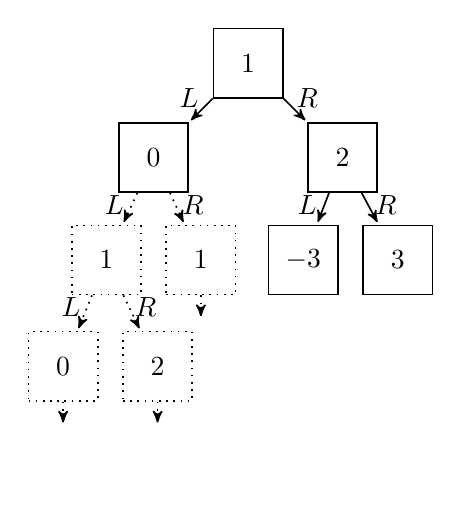
\begin{tikzpicture}[->,>=stealth',shorten >=1pt,auto,node distance=1.2cm,semithick]
\node[state,rectangle](q1){$1$};
\node[state,rectangle,white](q3)[below of=q1]{};
\node[state,rectangle](q2)[left of=q3]{$0$};
\node[state,rectangle](q4)[right of=q3]{$2$};

\node[state,rectangle,dotted](q6) at (-.6,-2.5) {$1$};
\node[state,rectangle,dotted](q5)[left of=q6]{$1$};

\node[state,rectangle](q7) at (0.7,-2.5) {$-3$};
\node[state,rectangle](q8)[right of=q7]{$3$};

\node[state,rectangle,white](q11)[below of=q6]{};

\node[state,rectangle,dotted](q9) at (-2.35,-3.85) {$0$};
\node[state,rectangle,dotted](q10)[right of=q9]{$2$};

\node[state,rectangle,white](q12)[below of=q9] {$0$};
\node[state,rectangle,white](q13)[below of=q10]{$2$};

\draw[->](q1)edge[swap](q2);
\draw[->](q1)edge[swap](q4);
\draw[->](q2)edge[swap,dotted](q5);
\draw[->](q2)edge[swap,dotted](q6);
\draw[->](q4)edge[swap](q7);
\draw[->](q4)edge[swap](q8);

\draw[->](q5)edge[swap,dotted](q9);
\draw[->](q5)edge[swap,dotted](q10);
\draw[->](q6)edge[swap,dotted](q11);
\draw[->](q9)edge[swap,dotted](q12);
\draw[->](q10)edge[swap,dotted](q13);

\node at (-.75,-.45) {$L$};
\node at (.75,-.45) {$R$};
\node at (-1.7,-1.8) {$L$};
\node at (-0.7,-1.8) {$R$};
\node at (1.75,-1.8) {$R$};
\node at (0.75,-1.8) {$L$};
\node at (-2.25,-3.1) {$L$};
\node at (-1.3,-3.1) {$R$};
\end{tikzpicture}

\caption{\small The (pseudo) execution paths of MPP~(\ref{eqn:eg-wnt}) on input $x=1$}\label{fig:eg-wnt}
\end{minipage}
\end{figure}

\begin{example}\label{eg:wnt}
Consider the following MPP
\begin{equation}\label{eqn:eg-wnt}
\while \quad ((x-1)(x-2)=0) \quad \left\{
\begin{array}{ll}
& \quad x := 1-x^2; \\
\,|| & \quad x := x+1; \\
\end{array}
\,\right\} \enspace .
\end{equation}
We associate symbols $L,R$ with the first and second assignments, respectively. Note that the loop guard is satisfied if and only if $x=1$ or $x=2$. Then it is easy to verify that $x=1$ is a weak non-terminating input of MPP~(\ref{eqn:eg-wnt}), by choosing $\tau_k$ as $\epsilon, R, LL, LLR, LLLL, \ldots$ (see Figure~\ref{fig:eg-wnt}).
Note that $x=1$ is actually a terminating input of MPP~(\ref{eqn:eg-wnt}) and the dotted nodes in Figure~\ref{fig:eg-wnt} cannot be reached by real execution. \rulex
\end{example}

Denote the set of all strong non-terminating inputs and weak non-terminating inputs by $\SNTI$ and $\WNTI$, respectively. Then the relationship between the above notions of non-termination can be stated as the following proposition.

\begin{proposition}\label{prop:3-termination}
For MPP~(\ref{eqn:MPP}), the inclusions $\SNTI \subseteq \NTI \subseteq \WNTI$ hold.
\end{proposition}
\begin{proof}
The first inclusion follows from $\Sigma^{\omega} \subseteq {\bf Path}(\xx) \Longrightarrow \Sigma^{\omega} \cap {\bf Path}(\xx) \neq \emptyset$. Second, for any $\xx \in \NTI$, there exists $\tau \in \Sigma^{\omega}$ satisfying the condition of Definition~\ref{dfn:exe-path}. Then by choosing $\tau_k$ as the prefix of $\tau$ with length $k$, we can see from (\ref{eqn:wnt}) that $\xx \in \WNTI$. Thus $\NTI$ is a subset of $\WNTI$. \rulex
\end{proof}

\begin{remark}
Both inclusions in Proposition~\ref{prop:3-termination} may be proper: from Examples~\ref{eg:exe-path} and \ref{eg:nt} we can see that $(1,-1) \in \NTI$, but $(1,-1) \notin \SNTI$ for MPP~(\ref{eqn:eg-exe-path}); Example~\ref{eg:wnt} shows that $1 \in \WNTI$, but $1 \notin \NTI$ for MPP~(\ref{eqn:eg-wnt}). However, if MPP~(\ref{eqn:MPP}) has a single path, we can conclude that $\SNTI=\NTI=\WNTI$.
\end{remark}

According to Proposition~\ref{prop:3-termination}, strong/weak non-termination can be used in under/over approximation analysis of non-termination: any element in $\SNTI$ is a witness to the non-termination of MPP~(\ref{eqn:MPP}), and conversely the emptiness of $\WNTI$ implies that MPP~(\ref{eqn:MPP}) terminates on all inputs.


\section{The Computation of SNTI}\label{sec:snt}
In this section, based on polynomial ideal theory, we will reduce $\SNTI$ of any MPP~(\ref{eqn:MPP}) to the real variety of a polynomial ideal $\I$; furthermore, we can always compute a finite basis of $\I$, thus giving a complete characterization of $\SNTI$. This enables us to check the emptiness of $\SNTI$ for any MPP~(\ref{eqn:MPP}), or test whether $\xx \in \SNTI$ for a given $\xx \in \mathbb{R}^n$.

\subsection{Iteration Trees}\label{sec:it-tree}
During the execution of MPPs, the assignments ${\bf A}_i$ in the loop body are applied to program states $\xx$. On the other hand, if we focus on the loop guard test of each iteration, the assignments can also be viewed as applications to the loop guard $G(\xx)=0$, which produce a series of polynomial equations, or equivalently, polynomials. Using these polynomials as nodes, we can construct an \emph{iteration tree} (see Figure~\ref{fig:it-tree}) which is very useful in the computation of non-terminating inputs.

\begin{definition}[Iteration Tree]\label{dfn:it-tree}
An \emph{iteration tree} of MPP~(\ref{eqn:MPP}) is defined inductively as:
\begin{itemize}
\item the \emph{root} is $G(\xx)$, i.e., the polynomial in the loop guard of MPP~(\ref{eqn:MPP});
\item for any node $G({\bf p}(\xx))$ in the tree, where ${\bf p}(\xx): \mathbb{R}^n \rightarrow \mathbb{R}^n$ is a vector function, it has $\ell$ directly successive nodes $G({\bf A}_1({\bf p}(\xx))),G({\bf A}_2({\bf p}(\xx))),\ldots,G({\bf A}_{\ell} ({\bf p}(\xx)))$; and there is a \emph{directed edge} connecting $G({\bf p}(\xx))$ and $G({\bf A}_i ({\bf p}(\xx)))$, labeled by $a_i$, for any $1 \leq i \leq \ell$.
\end{itemize}
\end{definition}

\begin{figure}
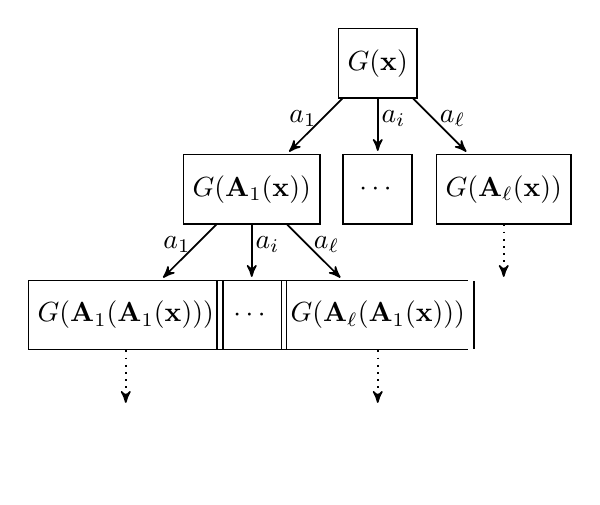
\begin{tikzpicture}[->,>=stealth',shorten >=1pt,auto,node distance=1.6cm,semithick]
\node[state,rectangle](q1){$G(\xx)$};
\node[state,rectangle](q3)[below of=q1]{$\cdots$};
\node[state,rectangle](q2)[left of=q3]{$G({\bf A}_1(\xx))$};
\node[state,rectangle](q4)[right of=q3]{$G({\bf A}_{\ell}(\xx))$};
\node[state,rectangle](q6)[below of=q2]{$\cdots$};
\node[state,rectangle](q5)[left of=q6]{$G({\bf A}_1({\bf A}_1(\xx)))$};
\node[state,rectangle](q7)[right of=q6]{$G({\bf A}_{\ell}({\bf A}_1(\xx)))$};

\node[state,rectangle,white](q8)[below of=q4]{};
\node[state,rectangle,white](q9)[below of=q5]{};
\node[state,rectangle,white](q10)[below of=q7]{};

\draw[->](q1)edge[swap](q2); \draw[->](q1)edge[swap](q3);
\draw[->](q1)edge[swap](q4); \draw[->](q2)edge[swap](q5);
\draw[->](q2)edge[swap](q6); \draw[->](q2)edge[swap](q7);
\draw[->](q4)edge[swap,dotted](q8);
\draw[->](q5)edge[swap,dotted](q9);
\draw[->](q7)edge[swap,dotted](q10);

\node at (-.95,-.7) {$a_1$};
\node at (.2,-.7) {$a_i$};
\node at (.95,-.7) {$a_{\ell}$};
\node at (-2.55,-2.3) {$a_1$};
\node at (-1.4,-2.3) {$a_i$};
\node at (-.65,-2.3) {$a_{\ell}$};
\end{tikzpicture}
\caption{\small The iteration tree of MPP~(\ref{eqn:MPP})}\label{fig:it-tree}
\end{figure}

\begin{remark}
Iteration trees have the following features compared with execution trees:
\begin{itemize}
\item each node in an iteration tree is a polynomial in $\mathbb{Q}[\xx]$, rather than an element in $\mathbb{R}^n$;
\item iteration trees are infinite trees with no leaf node, and each node has exactly $\ell$ children;
\item an iteration tree is constructed statically without dynamically executing an MPP to get the trace of program state variables.
\end{itemize}
\end{remark}

\subsection{Computing SNTI as Real Varieties}
Intuitively, a strong non-terminating input $\xx \in \mathbb{R}^n$ of an MPP will persistently satisfy the loop guard $G(\xx)=0$, and thus must be a common real root of all the polynomials in the iteration tree of the MPP. To see this, it is convenient to consider the infinitely many polynomials in an iteration tree level by level, rather than by paths.
\begin{lemma}\label{lem:snt-1}
\[
\SNTI=\V\left( \bigcup_{k \geq 0} \bigcup_{|\tau|=k} \{G(\A_{\tau}(\xx))\} \right) \cap \mathbb{R}^n \enspace .
\]
\end{lemma}
\begin{proof}
By Definition~\ref{def:SNT}, $\xx \in \SNTI$ if and only if for any $\tau \in \Sigma^{\omega}$, and any $\tau' \in {\bf Pre}(\tau)$, $G(\A_{\tau'}(\xx))=0$, i.e.,
\[
\SNTI=\V\left( \bigcup_{\tau \in \Sigma^{\omega}} \bigcup_{\tau' \in {\bf Pre}(\tau)} \{G(\A_{\tau'}(\xx))\} \right) \cap \mathbb{R}^n \enspace .
\]
Hence this lemma follows immediately from the fact
\[
\bigcup_{\tau \in \Sigma^{\omega}} \bigcup_{\tau' \in {\bf Pre}(\tau)} \{\tau'\} = \bigcup_{k \geq 0} \bigcup_{|\tau|=k} \{\tau\} \enspace .
\]
\rulex
\end{proof}

To employ the correspondence between ideals and varieties and the nice properties of polynomial ideals, let
\begin{equation}\label{eqn:ideal-snt}
\I_k \,\,\define\,\left\langle \bigcup_{|\tau| \leq k} \{G(\A_{\tau}(\xx))\} \right\rangle \qquad (k=0,1,2,\ldots) \enspace .
\end{equation}
That is, $\I_k$ is the ideal generated by all the polynomials from the top $k+1$ levels of the iteration tree. Then we have
\begin{lemma}\label{lem:snt-2}
\[
\SNTI=\V\left( \bigcup_{k \geq 0} \I_k \right) \cap \mathbb{R}^n \enspace .
\]
\end{lemma}
\begin{proof}
By (\ref{eqn:ideal-snt}) it is easy to show that
\[
\bigcup_{k \geq 0}\I_k = \bigcup_{k \geq 0} \left\langle \bigcup_{|\tau| \leq k} \{G(\A_{\tau}(\xx))\} \right\rangle = \left\langle \bigcup_{k \geq 0} \bigcup_{|\tau| \leq k} \{G(\A_{\tau}(\xx))\} \right\rangle  = \left\langle \bigcup_{k \geq 0} \bigcup_{|\tau|=k} \{G(\A_{\tau}(\xx))\} \right\rangle \enspace .
\]
Hence this lemma follows from Lemma~\ref{lem:snt-1}. \rulex
\end{proof}

Lemma~\ref{lem:snt-2} can be further simplified to
\begin{lemma}\label{lem:snt-3}
There exists an integer $N \in \mathbb{N}$ such that
\[
\SNTI = \V(\I_N) \cap \mathbb{R}^n \enspace .
\]
\end{lemma}
\begin{proof}
Note that $\I_0 \subseteq \I_1 \subseteq \I_2 \subseteq \cdots$ forms an ascending chain of ideals. Hence this lemma follows from Theorem~\ref{ascending} and Lemma~\ref{lem:snt-2}. \rulex
\end{proof}

Now we have reduced $\SNTI$ of MPP~(\ref{eqn:MPP}) to the real variety of a polynomial ideal. The following theorem shows that the integer $N$ in Lemma~\ref{lem:snt-3} is actually computable.

\begin{theorem}[Fixed Point Theorem]\label{thm:fixed-snt}
If $\I_m=\I_{m+1}$, then $\I_m=\I_k$ for any $k \geq m+1$.
\end{theorem}
\begin{proof}
We prove this by induction on $k$ for $k \geq m+1$.

Basis: $\I_m=\I_{m+1}$, which means $G(\A_{\tau}(\xx)) \in \I_m$ for any $\tau$ with $|\tau| \leq m+1$.

Induction: Assume that $\I_m = \I_k$ for some $k \geq m+1$, which means for any $\tau$ with $|\tau|=k$, there exist $g_{\sigma}(\xx) \in \mathbb{Q}[\xx]$, for each $\sigma \in \Sigma^*$ with $|\sigma| \leq m$, such that
\[
G(\A_{\tau}(\xx))=\sum_{|\sigma| \leq m} g_{\sigma}(\xx) G(\A_{\sigma}(\xx)) \enspace .
\]
We will show that $\I_m = \I_{k+1}$. Note that for any $\tau$ with $|\tau|=k+1$, we have
\[
\begin{array}{lll}
G(\A_{\tau}(\xx)) & = G(\A_{\tail(\tau)}(\A_{\head(\tau)}(\xx))) & \quad(|\tail(\tau)|=k) \\
& = \sum\limits_{|\sigma|\leq m} g_{\sigma}(\A_{\head(\tau)}(\xx)) G(\A_{\sigma}(\A_{\head(\tau)}(\xx))) & \quad \mbox{(by induction hypothesis)} \\
& = \sum\limits_{|\sigma|\leq m} g_{\sigma}(\A_{\head(\tau)}(\xx)) G(\A_{\head(\tau)\cdot\sigma}(\xx)) & \quad (|\head(\tau) \cdot \sigma| \leq m+1) \\
& \in \,\I_m & \quad (\mbox{by induction basis}) \enspace .
\end{array}
\]
\rulex
\end{proof}

By Theorem~\ref{thm:fixed-snt}, $N$ can be computed as the first integer $k$ satisfying $\I_k=\I_{k+1}$. Now the main result on $\SNTI$ computation can be stated as:
\begin{theorem}\label{thm:main-snt}
For MPP~(\ref{eqn:MPP}), an integer $N \in \mathbb{N}$ can be computed such that
\[
\SNTI=\V(\I_N) \cap \mathbb{R}^n \enspace .
\]
\end{theorem}
\begin{proof}
It follows immediately from Lemma~\ref{lem:snt-3} and Theorem~\ref{thm:fixed-snt}. \rulex
\end{proof}

An abstract algorithm for computing $\SNTI$ can be given as:
\begin{algorithm}\label{alg:snt}
$k \leftarrow 0$\;
\While{$\I_{k} \neq \I_{k+1}$}
    {$k \leftarrow k+1$\;}
    {\KwRet{$\V(\I_k) \cap \mathbb{R}^n$}\;}
\caption{The Computation of $\SNTI$ for MPP~(\ref{eqn:MPP})}
\end{algorithm}

\begin{example} \label{eg:computation-snt}
We show the application of Algorithm~\ref{alg:snt} to three aforementioned MPPs.
\begin{enumerate}
\item[1)] For MPP~(\ref{eqn:eg-exe-path}), we get\footnote{For the computation of Gr\"obner bases, we are assuming the \emph{pure lexicographic order} $x \succ y$.}
    \[
    \I_0=\langle x+y \rangle \subsetneq \I_1=\langle y^2,x+y \rangle \subsetneq \I_2=\langle 1 \rangle = \I_3 \enspace .
    \]
    So $\SNTI = \V(\langle 1 \rangle) \cap \mathbb{R}^2 = \emptyset$.
\item[2)] For MPP~(\ref{eqn:eg-snt}), we get
    \[
    \I_0=\langle x^2+1-y \rangle \subsetneq \I_1=\langle y^2-2y,x^2+1-y \rangle = \I_2 \enspace .
    \]
    So $\SNTI=\V(\langle y^2-2y,x^2+1-y \rangle) \cap \mathbb{R}^2=\{(1,2),(-1,2)\}$.
\item[3)] For MPP~(\ref{eqn:eg-wnt}), we get
    \[
    \I_0=\langle x^2-3x+2 \rangle \subsetneq \I_1=\langle 1 \rangle = \I_2 \enspace .
    \]
    So $\SNTI=\V(\langle1\rangle) \cap \mathbb{R}=\emptyset$. \rulex
\end{enumerate}
\end{example}


\section{The Computation of WNTI}\label{sec:wnt}
In this section, we will first reduce $\WNTI$ of MPP~(\ref{eqn:MPP}) to the real variety of a certain polynomial ideal $\J$. We then provide a \emph{sufficient} criterion under which a finite basis of $\J$ can be computed, and thus give a complete characterization of $\WNTI$ under such a criterion.

\subsection{Identifying WNTI as Real Varieties}
Intuitively, a weak nonterminating input is a real root of at least one of the polynomials at every level of the iteration tree in Figure~\ref{fig:it-tree}, or equivalently, a real root of the \emph{product} of the polynomials (called a \emph{product polynomial}) at each level.

\begin{lemma}\label{lem:wnt-1}
\[
\WNTI=\V\left(\bigcup_{j \geq 0} \left\{\prod_{|\tau|=j} G(\A_{\tau}(\xx)) \right\} \right) \cap \mathbb{R}^n \enspace .
\]
\end{lemma}
\begin{proof}
It is a direct translation of (\ref{eqn:wnt}) in Definition~\ref{def:WNT}. \rulex
\end{proof}

To adopt the language of polynomial ideals, we consider the ideals generated by the \emph{product polynomials} from the top $k+1$ levels of the iteration tree:
\begin{equation}\label{eqn:ideal-wnt}
\J_k\,\,\define\,\left\langle \bigcup_{j \leq k} \left\{ \prod_{|\tau|=j} G(\A_{\tau}(\xx)) \right\} \right\rangle \qquad (k=0,1,2,\ldots) \enspace .
\end{equation}
Then we have
\begin{lemma}\label{lem:wnt-2}
\[
\WNTI=\V\left(\bigcup_{k \geq 0} \J_k \right) \cap \mathbb{R}^n \enspace .
\]
\end{lemma}
\begin{proof}
By (\ref{eqn:ideal-wnt}) it is easy to show that
\[
\begin{array}{ll}
\bigcup\limits_{k \geq 0} \J_k & = \bigcup\limits_{k \geq 0} \left\langle \bigcup\limits_{j \leq k} \left\{ \prod\limits_{|\tau|=j} G(\A_{\tau}(\xx)) \right\} \right\rangle = \left\langle \bigcup\limits_{k \geq 0} \bigcup\limits_{j \leq k} \left\{ \prod\limits_{|\tau|=j} G(\A_{\tau}(\xx)) \right\} \right\rangle \\
& = \left\langle \bigcup\limits_{j \geq 0} \left\{ \prod\limits_{|\tau|=j} G(\A_{\tau}(\xx)) \right\} \right\rangle \enspace .
\end{array}
\]
Hence this lemma follows from Lemma~\ref{lem:wnt-1}. \rulex
\end{proof}

Lemma~\ref{lem:wnt-2} can be further simplified to
\begin{lemma}\label{lem:wnt-3}
There exists an integer $N \in \mathbb{N}$ such that
\[
\WNTI=\V(\J_N) \cap \mathbb{R}^n \enspace .
\]
\end{lemma}
\begin{proof}
Note that $\J_0 \subseteq \J_1 \subseteq \J_2 \subseteq \cdots$ forms an ascending chain of ideals. Hence this lemma follows from Theorem~\ref{ascending} and Lemma~\ref{lem:wnt-2}. \rulex
\end{proof}

Now we have proved that $\WNTI$ of MPP~(\ref{eqn:MPP}) is a real variety, a result analogous to what we have established for $\SNTI$ (Lemma~\ref{lem:snt-3}). However, we do not have a criterion like Theorem~\ref{thm:fixed-snt} for checking the fixed point of the chain of ideals $\J_k$. Nevertheless, a \emph{sufficient} criterion will be given under some conditions in the coming subsection.

\subsection{A Sufficient Criterion for Computability of WNTI}
Let \begin{equation}\label{eqn:ideal-wnt-trunc}
\hat{\J}_{m,k}\,\,\define\,\left\langle \bigcup_{m \leq j \leq k}\left\{ \prod_{|\tau|=j} G(\A_{\tau}(\xx)) \right\} \right\rangle \qquad (0 \leq m \leq k) \enspace .
\end{equation}
Intuitively, $\hat{\J}_{m,k}$ is the ideal generated by the \emph{product polynomials} from levels $m$ to $k$ in the iteration tree in Figure~\ref{fig:it-tree}.

For the ideals $\hat{\J}_{m,k}$ and $\J_k$ defined in (\ref{eqn:ideal-wnt-trunc}) and (\ref{eqn:ideal-wnt}) respectively, we have $\hat{\J}_{m,k} \subseteq \J_k$ for any $k \geq m \geq 0$, in particular, $\hat{\J}_{0,k}=\J_k$ for any $k \geq 0$. Besides, noticing that for any $m \in \mathbb{N}$, the sequence of $\hat{\J}_{m,k}$ for $k=m,m+1,m+2,\ldots$ forms an ascending chain of ideals, we can actually prove
\begin{lemma}\label{lem:wnt-4}
For any $M,N \in \mathbb{N}$ with $M \leq N$, if $\hat{\J}_{M,N}$ is the fixed point of the chain of ideals formed by $\{\hat{\J}_{M,k}\}|_{k \geq M}$, then $\J_N$ is the fixed point of the chain of ideals formed by $\{\J_k\}|_{k \geq 0}$.
\end{lemma}
\begin{proof}
It is sufficient to prove that for any $k> N$, $\hat{\J}_{M,N}=\hat{\J}_{M,k}$ implies $\J_N=\J_k$.

Note that $\hat{\J}_{M,N}=\hat{\J}_{M,k}$ implies
\[
\forall j. \,N<j \leq k: \quad \prod_{|\tau|=j} G(\A_{\tau}(\xx))\,\,\in \,\,\hat{\J}_{M,N}\,\,\subseteq\,\, \J_N  \enspace ,
\]
which means the set of generators of $\J_k$ are all elements of $\J_N$. Thus $\J_N=\J_k$. \rulex
\end{proof}

As mentioned above, for any $M \in \mathbb{N}$, how to compute the fixed point of the chain of ideals $\J_{M,k}$ for $k \geq M$ is an open problem in general. However, a sufficient criterion can be given as follows, which can be seen as a weak version of Theorem~\ref{thm:fixed-snt}.

\begin{theorem}[Weak Fixed Point Theorem]\label{thm:fixed-wnt}
If there exist $M,N \in \mathbb{N}$, $M\leq N$, such that $\hat{\J}_{M,N}$ is a principal ideal, i.e., $\hat{\J}_{M,N}=\langle H(\xx)\rangle$ for some $H(\xx) \in \mathbb{Q}[\xx]$, and in addition, $H(\xx)$ satisfies
\begin{equation}\label{eqn:principal-one-iteration}
\prod_{|\tau|=1} H(\A_{\tau}(\xx)) \ \in \ \langle H(\xx) \rangle \enspace ,
\end{equation}
then $\J_N=\J_k$ for all $k \geq N$.
\end{theorem}
\begin{proof}
By Lemma~\ref{lem:wnt-4}, it suffices to prove that $\hat{\J}_{M,N} = \hat{\J}_{M,k}$ for all $k \geq N$. The proof will proceed by induction on $k$ for $k \geq N$.

Suppose $\hat{\J}_{M,N}=\langle H(\xx) \rangle= \hat{\J}_{M,k}$ for some $k \geq N$. Then there exists $g(\xx) \in \mathbb{Q}[\xx]$ such that $\prod_{|\tau|=k} G(\A_{\tau}(\xx)) = g(\xx)H(\xx)$.
\[
\begin{array}{lll}
\prod\limits_{|\tau|=k+1} G(\A_{\tau}(\xx)) & = \prod\limits_{|\tau_1|=1}\, \prod\limits_{|\tau_2|=k} G(\A_{\tau_2}(\A_{\tau_1}(\xx))) \\
& = \prod\limits_{|\tau_1|=1} g(\A_{\tau_1}(\xx)) H(\A_{\tau_1}(\xx)) & \qquad \mbox{(by induction hypothesis)} \\
& = \left[ \prod\limits_{|\tau_1|=1} g(\A_{\tau_1}(\xx)) \right] \, \left[ \prod\limits_{|\tau_1|=1} H(\A_{\tau_1}(\xx)) \right] \\
& \in \langle H(\xx) \rangle & \qquad \mbox{(by the requirement~(\ref{eqn:principal-one-iteration}))} \enspace .
\end{array}
\]
Hence we get $\hat{\J}_{M,N}= \hat{\J}_{M,k+1}$, which completes the proof by induction. \rulex
\end{proof}

Now the main result on $\WNTI$ computation can be stated as follows, which is analogous to Theorem~\ref{thm:main-snt}.

\begin{theorem}\label{thm:main-wnt}
For MPP~(\ref{eqn:MPP}), if the requirements in Theorem~\ref{thm:fixed-wnt}  are satisfied, an integer $N$ can be computed such that
\[
\WNTI=\V(\J_N) \cap \mathbb{R}^n \enspace .
\]
\end{theorem}
\begin{proof}
It follows immediately from Lemma~\ref{lem:wnt-3} and Theorem~\ref{thm:fixed-wnt}. \rulex
\end{proof}

\subsection{Applying Theorem~\ref{thm:main-wnt} to Compute WNTI}
Based on Theorem~\ref{thm:main-wnt}, we present an abstract algorithm for computing $\WNTI$ of MPP~(\ref{eqn:MPP}):
\begin{algorithm}\label{alg:wnt}
$m \leftarrow 0$\;
\While{$m\leq M$}{
    $k \leftarrow m$\;
    \While{$\hat{\J}_{m,k} \neq \hat{\J}_{m,k+1}$}
    {$k \leftarrow k+1$\;}
    \eIf{$\hat{\J}_{m,k}=\langle H(\xx)\rangle$ \rm{and} $H(\xx)$ \rm{satisfies (\ref{eqn:principal-one-iteration})}}
    {\KwRet{$\V(\J_k) \cap \mathbb{R}^n$}\;}
    {$m \leftarrow m+1$\;}}
\KwRet{\sf unknown};
\caption{The Computation of $\WNTI$ for MPP~(\ref{eqn:MPP})}
\end{algorithm}

The meaning of Algorithm~\ref{alg:wnt} is: for each $m \in \mathbb{N}$, we compute $\hat{\J}_{m,k}$ for $k=m,m+1,m+2,\ldots$ until $\hat{\J}_{m,k}=\hat{\J}_{m,k+1}$ (lines 3--5)\footnote{By Theorem~\ref{ascending}, this iteration must terminate.}; then we test whether $\hat{\J}_{m,k}$ is a principal ideal and the single generator satisfies (\ref{eqn:principal-one-iteration}) (line 6); if the test succeeds, by Theorem~\ref{thm:main-wnt} we get the $\WNTI$ (line 7); otherwise, we increase $m$ by 1 (line 9) and continue the computation; the number $M$ in line 2 is a prescribed bound on $m$ to ensure termination of the whole algorithm, and when $m$ exceeds $M$, Algorithm~\ref{alg:wnt} terminates with the answer {\sf unknown} (line 10).

\begin{example}\label{eg:computation-wnt}
We use Algorithm~\ref{alg:wnt} to compute the $\WNTI$ of several MPPs.
\begin{enumerate}
\item[1)] For MPP~(\ref{eqn:eg-exe-path}), we get $\hat{\J}_{0,0}= \langle x+y \rangle = \hat{\J}_{0,1}$, in which $x+y$ satisfies (\ref{eqn:principal-one-iteration}). So $\WNTI = \V(\J_0) \cap \mathbb{R}^2 = \V(\langle x+y \rangle) \cap \mathbb{R}^2$.
\item[2)] For MPP~(\ref{eqn:eg-snt}), we get $\hat{\J}_{0,0} = \langle x^2+1-y \rangle = \hat{\J}_{0,1}$, in which $x^2+1-y$ satisfies (\ref{eqn:principal-one-iteration}). So $\WNTI = \V(\J_0) \cap \mathbb{R}^2 = \V(\langle x^2+1-y \rangle) \cap \mathbb{R}^2$.
\item[3)] For MPP~(\ref{eqn:eg-wnt}), we get
     \[
     \hat{\J}_{1,1} = \langle x^4+x^6-x^3-x^5 \rangle \subsetneq \hat{\J}_{1,2} = \langle x^4-x^3 \rangle = \hat{\J}_{1,3} \enspace ,
     \]
     in which $x^4-x^3$ satisfies (\ref{eqn:principal-one-iteration}). So $\WNTI = \V(\J_2) \cap \mathbb{R} = \V(\langle x-1 \rangle) \cap \mathbb{R} = \{1\}$.
\item[4)] Consider the following MPP
    \begin{equation}\label{eqn:eg-wnt-empty}
    \while \quad (x-y^2=0) \quad \left\{
    \begin{array}{ll}
    & \quad (x,y) := (x+3,y+1); \\
    || & \quad (x,y) := (1,0); \\
    \end{array}
    \right\} \enspace .
    \end{equation}
    We can get
    \[
    \hat{\J}_{0,0} = \langle x-y^2 \rangle \subsetneq \hat{\J}_{0,1} = \langle y-1,x-1 \rangle \subsetneq \hat{\J}_{0,2} = \langle 1 \rangle = \hat{\J}_{0,3} \enspace .
    \]
    So $\WNTI = \V(\J_2) \cap \mathbb{R}^2 = \V(\langle 1 \rangle) \cap \mathbb{R}^2 = \emptyset$, which further implies $\NTI=\SNTI=\emptyset$. \rulex
\end{enumerate}
\end{example}

The results of Examples~\ref{eg:computation-snt} and \ref{eg:computation-wnt} can be summarized in Table~\ref{tbl:snt-wnt-nt}.
\begin{table}
\begin{center}
\caption{\small A summary of the computation of non-terminating inputs}\label{tbl:snt-wnt-nt}
\vskip 1mm
\begin{tabular}{|c|c|c|c|c|}
  \hline
  MPP & (\ref{eqn:eg-exe-path}) & (\ref{eqn:eg-snt}) & (\ref{eqn:eg-wnt}) & (\ref{eqn:eg-wnt-empty}) \\
  \hline
  $\SNTI$ & $\emptyset$ & $\{(1,2),\,(-1,2)\}$ & $\emptyset$ & $\emptyset$ \\
  $\NTI$ & ? & $\supseteq \{(1,2),\,(-1,2)\} $ & ? & $\emptyset$ \\
  $\WNTI$ & $\V(\langle x+y\rangle) \cap \mathbb{R}^2$ & $\V(\langle x^2+1-y \rangle ) \cap \mathbb{R}^2$ & $\{1\}$ & $\emptyset$ \\
  \hline
\end{tabular}
\end{center}
\end{table}

We explain a bit about the row corresponding to $\NTI$ in Table~\ref{tbl:snt-wnt-nt}. For MPP~(\ref{eqn:eg-snt}), it can be inferred that $\NTI$ is a superset of $\{(1,2),\,(-1,2)\}$ and must be nonempty. For MPP~(\ref{eqn:eg-wnt-empty}), the emptiness of $\WNTI$ implies the emptiness of $\NTI$. For MPPs~(\ref{eqn:eg-exe-path}) and (\ref{eqn:eg-wnt}), we cannot infer any information from the $\SNTI$/$\WNTI$-approximations and therefore the $\NTI$ are marked with ``?''. Actually from the analysis of Examples~\ref{eg:snt} and \ref{eg:wnt} we have known that $(1,-1)$ is in the $\NTI$ of MPP~(\ref{eqn:eg-exe-path}), while the $\NTI$ of MPP~(\ref{eqn:eg-wnt}) is empty.


\section{Conclusion}\label{sec:conc}
In this paper, we studied the detection of non-terminating inputs over $\mathbb{R}$ for multi-path polynomial programs with equational loop guards (MPP~(\ref{eqn:MPP})). We first defined on MPP the notions of non-terminating inputs ($\NTI$) as well as its under/over-approximation, i.e., strong/weak non-terminating inputs ($\SNTI$/$\WNTI$). Then based on the well-known theory of polynomial ideals, we presented a complete approach for computing $\SNTI$, and a sound but incomplete approach for computing $\WNTI$, both as the real variety of a certain polynomial ideal. Once the $\SNTI$/$\WNTI$ are computed, useful information on $\NTI$ can be inferred.

We have experimented with the proposed algorithms on several simple examples, by interactively calling existing functions in the {\sc Maple} environment. We did these experiments mainly with the purpose of testing and demonstrating proposed algorithms. A fully automated tool with applications to real programs is not provided, due to the high complexity of our approach: the polynomial ideal membership problem is \emph{exponential space complete} in the size of the problem instance \cite{mayr:EXPSC}, and the computation of Gr\"obner basis has even higher worst case complexity; besides, for MPPs with more than one paths, the sizes of ideals $\I_k$ or $\J_k$ in our algorithm grow exponentially with $k$, which could be very large when the fixed point is reached. An estimation of how large $k$ could eventually be is required for a more precise complexity analysis.

There are two theoretical problems left open in this paper:
\begin{enumerate}
\item[1)] Can we drop the restrictive assumption on $\WNTI$ computation and give a complete algorithm for computing $\WNTI$?
\item[2)] Is $\NTI$ reducible to the real variety of a polynomial ideal? If so, how can this variety be computed (at least under some restrictions)?
\end{enumerate}
A negative conjecture could be that a complete description of $\WNTI$ or $\NTI$ is not computable for MPP~(\ref{eqn:MPP}) in general. We are interested in answering these questions in future.


\acknowledgements{\rm We thank Professors Chaochen Zhou, Lu Yang, Zhibin Li, Bican Xia, Mingsheng Wang and Dingkang Wang for their beneficial discussions on our work. We also thank anonymous reviewers for their valuable comments on the revision of this paper.}


\bibliographystyle{spbasic}
\bibliography{template}

\end{document}
